\begin{figure}[!]
    \centering
    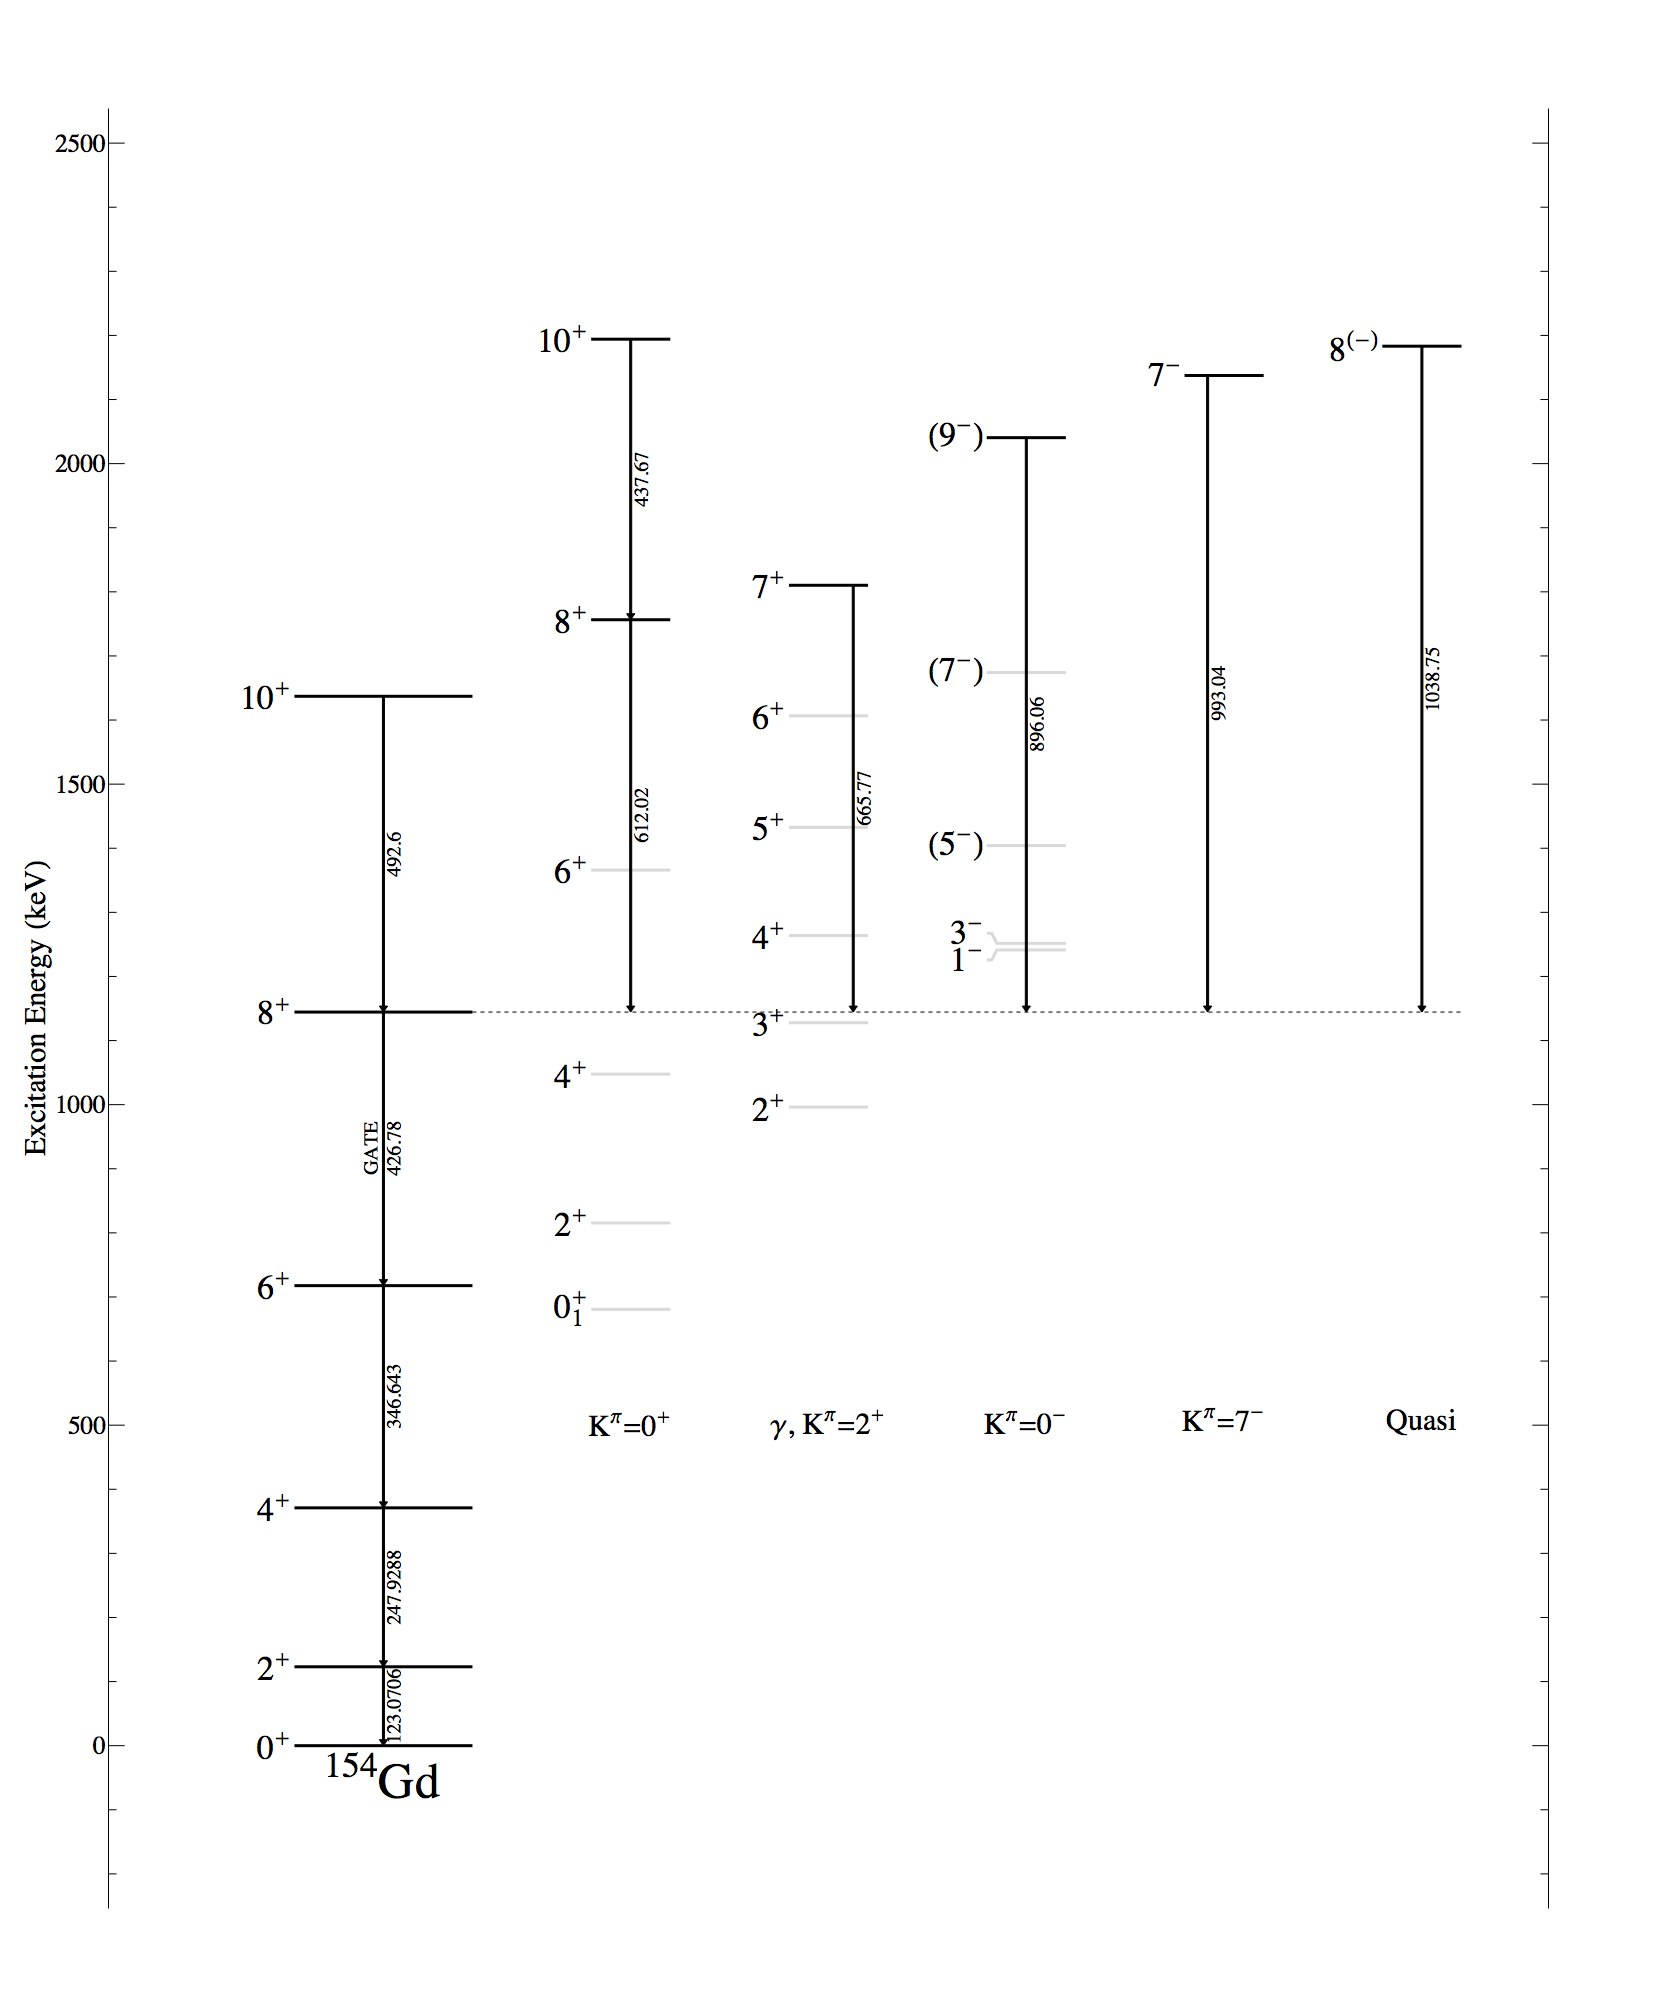
\includegraphics[scale=0.25]{154GdTablesAndFigs/154Gd_8to6.png}
    \caption{Level Scheme of $^{154}$Gd. The gamma ray of the $8^+\rightarrow6^+$ transition (426 keV) in the ground state was gated on. It was then compared with the gated spectrum from the gamma ray of the $10^+\rightarrow8^+$ transition (492 keV) in the ground state. Peaks only appearing in the first gate were assumed to go into the $8^+$ state, and assignments were made. Additionally, these peaks were also gated on, to look for cascades leading into the $8^+$ state, which were found in several cases. The levels are organized by band. The lower levels of the band, unseen by gamma rays in this gate, are in gray.}
    \label{fig:154_8to6}
\end{figure}